\documentclass[report.tex]{subfiles}

\begin{document}
\section{Results and Discussion}

The FEM simulation was successful in outputting all parameters (figure \ref{fig:FinalSimulationResults}), showing that the OOF2 program can handle multi-grain images with two sets of material parameters. The heat diffusion looks constant through the alpha and beta grains which is expected by their thermal conductivity values being similar. The x- and y- displacement contours are fairly consistent with previously generated results in the test cases, with the maximum displacement at 2.64 $\mu$m and 2.55 $\mu$m respectively. These displacement values are more similar than previous results, due to the image containing a more even quantity of alpha and beta and the coefficients of thermal expansion are more similar than the test cases.\\
\\ 
The FEM stress distribution for the Ti-6Al-4V image shows similar results to test case 4, where stress increases with decreasing temperature. The alpha regions show higher stress values relative to the beta regions at equivalent temperatures. Alpha Ti-6Al-4V has a lower coefficient of thermal expansion and hence the shrinkage with decreasing temperature is less significant, causing the stress to be higher. For this reason, there are stress concentrations at grain boundaries due to the shrinkage mismatch. This shows that the simulation is working well to give information about the stress distribution in the globular microstructure of Ti-6Al-4V.\\
\\
The simulation is limited in its usefulness as temperature dependent parameters have not been used. It also assumes that the Ti-6Al-4V microstructure is constant, when cooling from 1000 $\degree$C to 0 $\degree$C goes through the $\beta$-transus at 980 $\degree$C and the $\beta$ to metastable $\alpha$' at 800 $\degree$C \cite{Ti64PhaseDiagram}. The simulation was fixed on the left edge which may also affect the stress distribution in the microstructure.

\begin{figure}[h!]
    \centering
    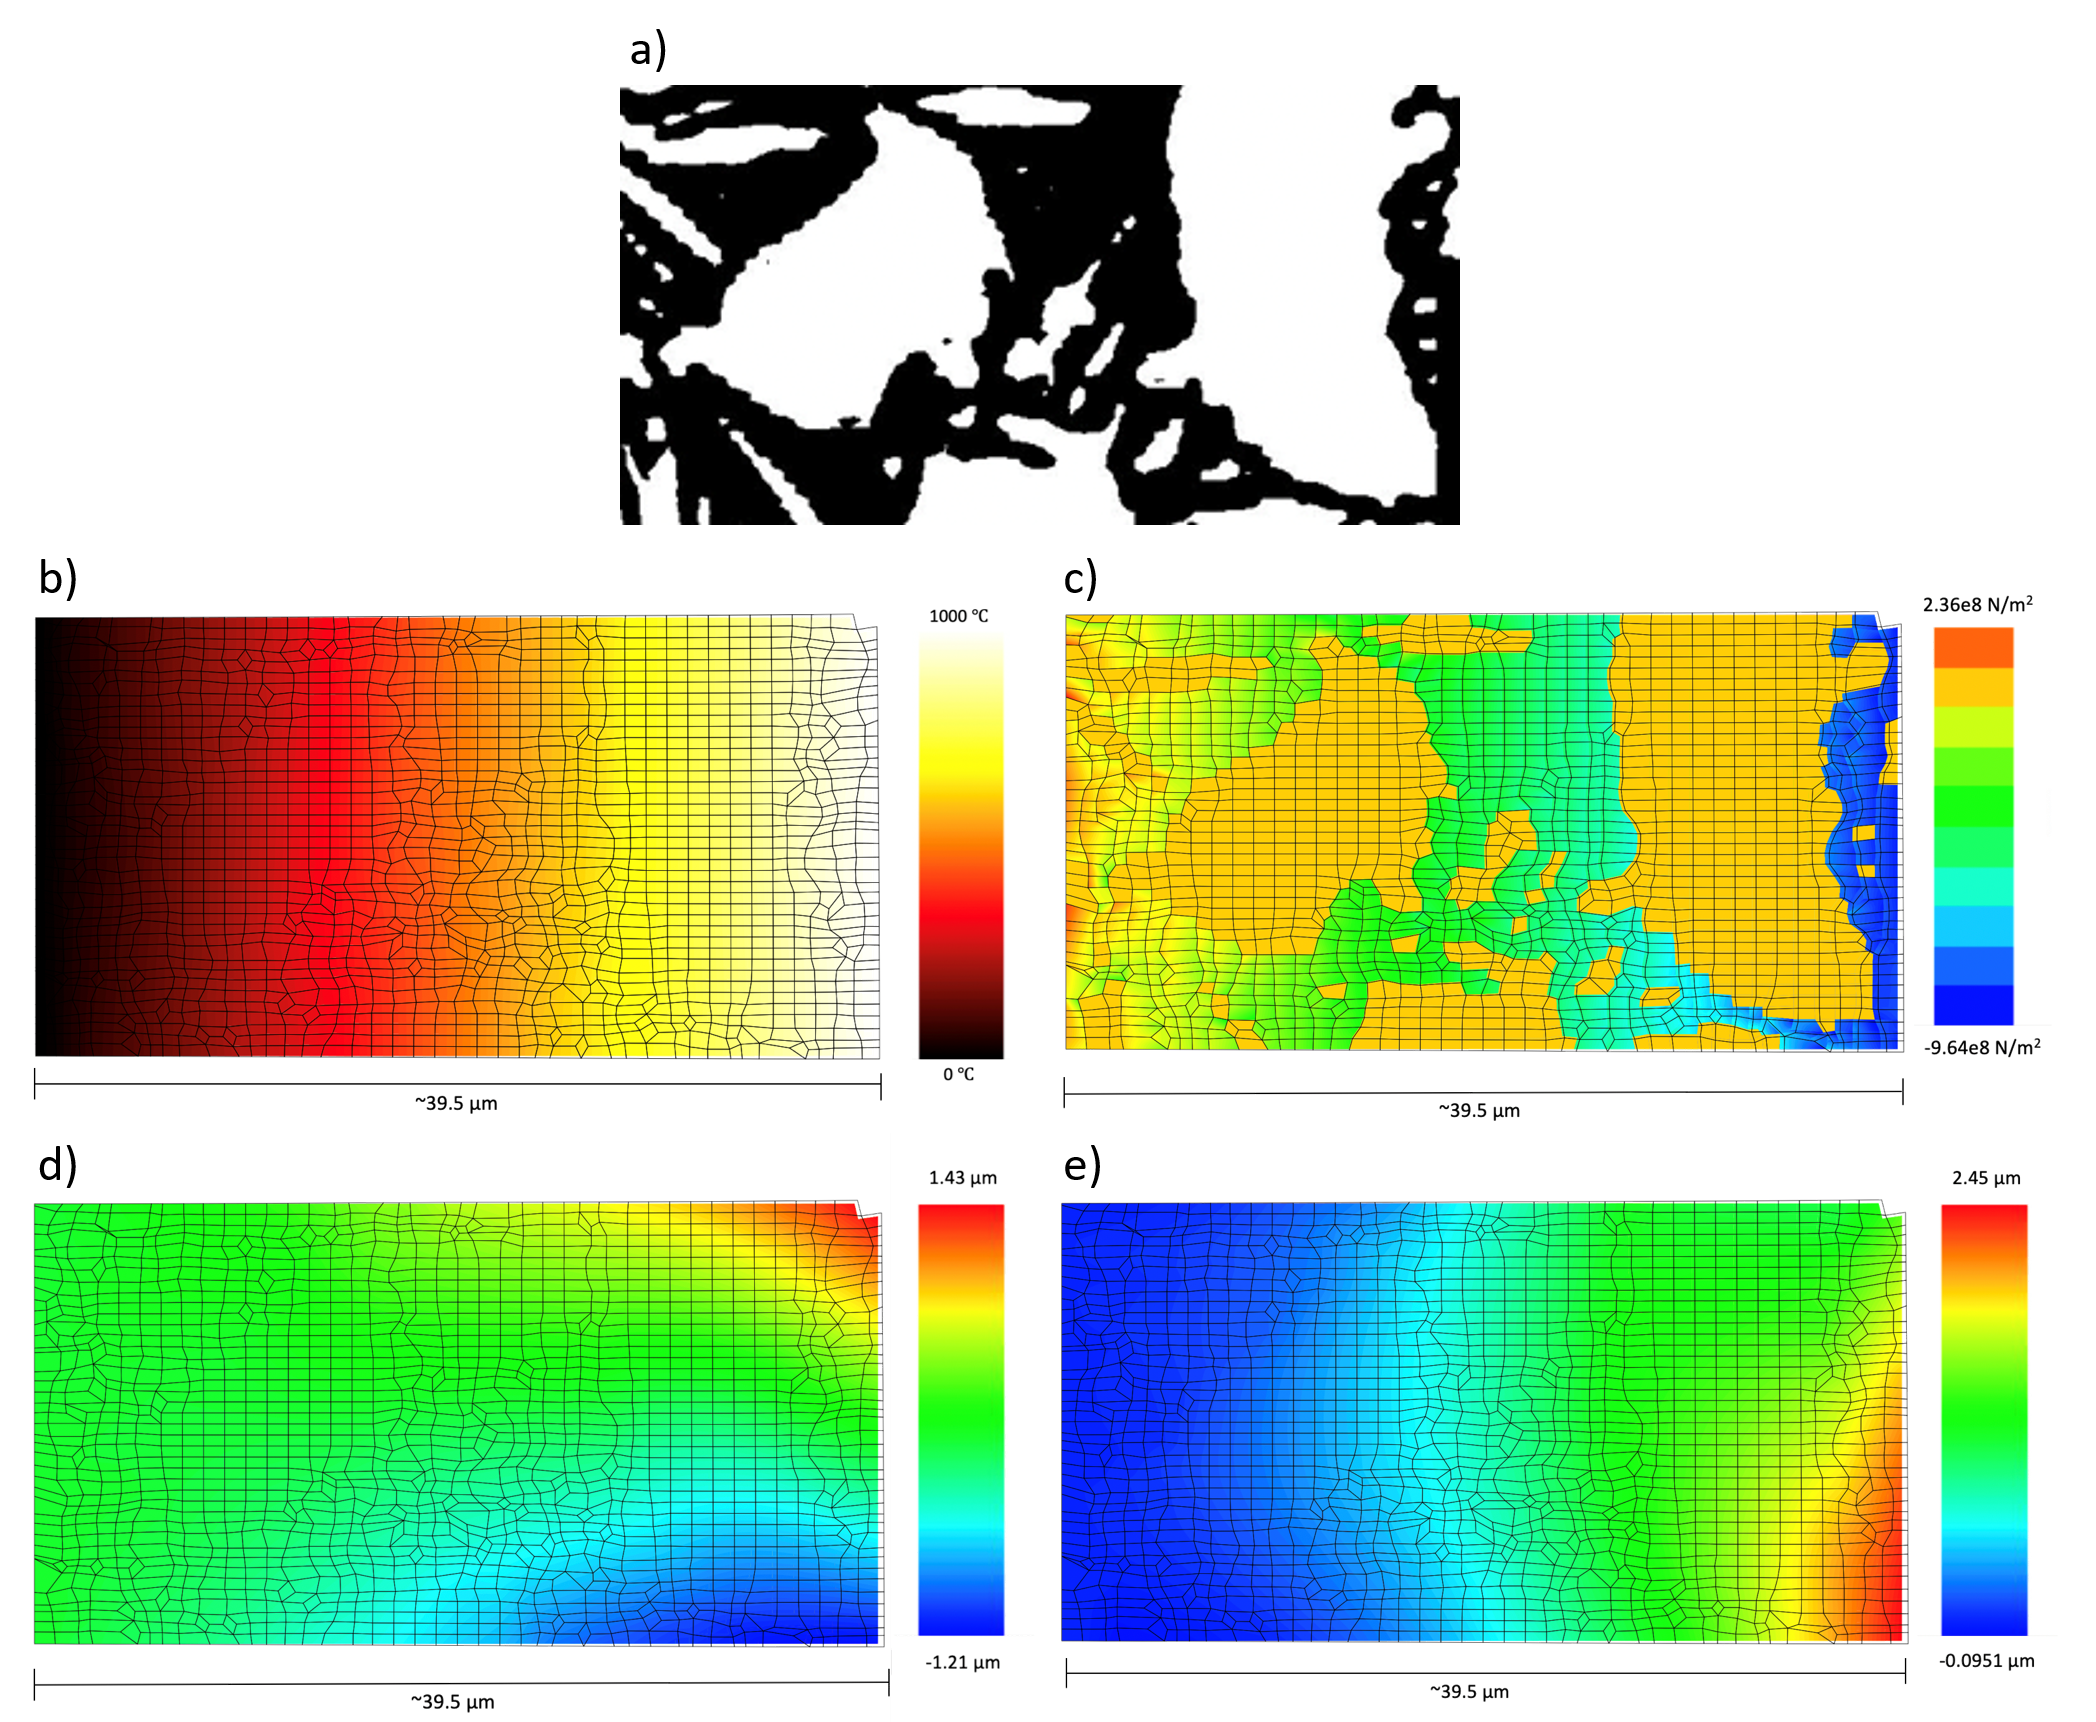
\includegraphics[width=17cm]{Ti64_Final_Simulation_Results.png}
    \caption{FEM simulation results, showing the a) original microstructure of Ti-6Al-4V b) heat diffusion through the grains c) stress    within the grains d) displacement in the x-direction e) displacement in y-direction}
    \label{fig:FinalSimulationResults}
\end{figure}


\end{document}
